\documentclass[final,hyperref={pdfpagelabels=false}]{beamer}
\usepackage[orientation=portrait,size=a0,scale=1.4]{beamerposter}
\usetheme{uclposter}


%\title[GVHD]{Quantifying the importance of target organ specific interactions in the aetiology of GVHD}
\title[GVHD]{Quantifying the importance of target organ interactions in GvHD}
\author[a]{Claire Winship, P. Santos E Sousa, S. Cire, C. Bennett, R. Chakraverty, V. Plagnol}
%\institute[ugi]{UCL Genetics Institute}
%\date{\today}

%\usepackage[orientation=landscape,size=a1]{beamerposter}

%\usetheme{uclposter}
%\useinnertheme{blockborder}
%\setbeamercolor{block body}{bg=white,fg=black}

%\title{Title of the Poster}
%\author{Author 1 and Author 2}
%\institute{%
  %Department of Statistical Science,
  %University College London
%}

\mode<presentation>
{
%  \usetheme{Berlin}
\usecolortheme{ucl}
\setbeamercolor{block body}{bg=white,fg=black}
}
\usepackage{times}
\usepackage{amsmath,amsthm, amssymb, latexsym}
\boldmath
\usepackage[english]{babel}
\usepackage[latin1]{inputenc}


\begin{document}

\begin{frame}{} 


\begin{columns}[t]
  \begin{column}{.26\linewidth}
    \begin{block}{Graft versus host disease}
\begin{itemize}
      \item Following BMT, donor immune cells may attack normal host tissue resulting in acute graft vs host disease (GvHD)
  \item Tissue damage by cytotoxic T cells leads to recruitment of other effector cells - increases tissue injury and self perpetuates GvHD
      \item GvHD target tissues include: skin, liver and GI tract
  \item Use of HLA-mismatched non-related donors a major risk factor
      \item Mice primary model animal for pre-clinical studies
      \end{itemize}
    \end{block}
\vspace{3cm}
    \begin{block}{The ImmGen project}
\begin{minipage}{0.45\textwidth}
 {\small     \begin{itemize}
      \item ImmGen defines gene expression/regulatory modules in murine immune cells based on similarities in expression profiles 
      \item Coarse modules: gene groups exhibiting broadly similar expression 
	\item Fine modules: gene groups with more defined expression profiles
\item Comparing differentially expressed gene lists to ImmGen - identify enriched modules (see adjacent example)
      \item Fisher's exact test facilitates the comparison of differentially expressed gene lists with ImmGen
      \end{itemize}}
\end{minipage}
\begin{minipage}{0.45\textwidth}
\begin{figure}[!thb]
   \includegraphics[width=10cm]{/cluster/project8/vyp/Winship_GVHD/claire/results/Miller2012.pdf}
   \caption{Taken from Miller et al, 2012}
\end{figure}
\end{minipage}
%\begin{itemize}
%\item Comparing differentially expressed gene lists to ImmGen - identify enriched modules (see example above)
 %     \item Fisher's exact test facilitates the comparison of differentially expressed gene lists with ImmGen
%\end{itemize}
    \end{block}
\vspace{3cm}
\begin{block}{Experimental overview}
  \begin{center}
  \includegraphics[width = 20cm]{/cluster/project8/vyp/Winship_GVHD/vincent/GVHD/poster/figs/GVHD_flowchart.png}
  \end{center}
\end{block}
\begin{itemize}
\item All datasets use gene expression for characterisation of T-cells, currently microarrays but transition to RNA-Seq in process.
\item Datasets marked in red are generated and presented in this poster.
\item Experimental work is ongoing for the other two datasets.
\end{itemize}
  \end{column}



%%%%%%%%%%%%%%%%%%%%%%%%%%%%%%%%%%%%%%%%%%%%%%%%%%%%%%%%%%%%%
  \begin{column}{.36\linewidth}
    \begin{block}{Assessing the role of antigen presenting Langerhans cell}
  {\bf Objective:} In a monoclonal model, evaluate the effect of depleting Langerhans cells on the gene expression of effector T cells found in the lymph nodes and in the skin.


\begin{center}
   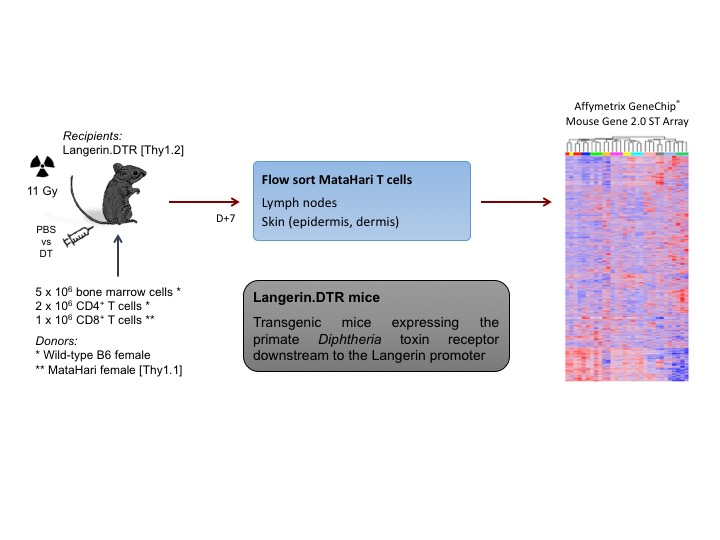
\includegraphics[width=25cm]{/cluster/project8/vyp/Winship_GVHD/vincent/GVHD/poster/figs/mataHari_DT.jpg}
\end{center}
\begin{itemize}
\item MataHari T cells: transgenic CD8 T cells that recognise a single ubiquitously-expressed male antigen (UTY peptide)
\item Tissues harvested at day +7 post BMT, MataHari T cells sorted and total RNA purified using Affymetrix GeneChip
\end{itemize}
    \end{block}
    \vspace{3cm}
    
    \begin{block}{Overview of results}
    
    
    \begin{itemize} % NOT SURE THIS IS NEEDED IF MODEL DIAGRAM IS INCLUDED
    \item Langerhans cells (LCs) are the predominant APCs in the skin and are radio-resistant  
    \item LCs have been shown to be sufficient for GvHD progression although this theory is controversial  
    \end{itemize}
      
    \hfill
    
    \begin{minipage}{0.6\textwidth}
      \includegraphics[width=17cm]{/cluster/project8/vyp/Winship_GVHD/claire/results/epi_dermis_PLN/figs/PCA_prettier.pdf}
    \end{minipage}
    \begin{minipage}{0.3\textwidth}
      {\small
	\begin{itemize}
	\item PCA plot shows tight cluster of DT treated samples - excludes epidermisDT
	\item Two samples (one dermis and one PLN) potential outliers but not extreme enough to be removed 
      \end{itemize}}
\end{minipage}
\end{block}
\vspace{3cm}

\begin{block}{How can we use ImmGen to understand these results?}  
\vspace{1cm}
\begin{minipage}{0.30\textwidth}
  \includegraphics[width=10cm]{/cluster/project8/vyp/Winship_GVHD/claire/results/epi_dermis_PLN/figs/epidermis_vs_epidermisDT_histogram.pdf}
\end{minipage}
\hfill
\begin{minipage}{0.30\textwidth}
    \includegraphics[width=10cm]{/cluster/project8/vyp/Winship_GVHD/claire/results/epi_dermis_PLN/figs/epidermis_vs_epidermisDT_coarse_module_association_graph.pdf}
\end{minipage}
\hfill
\begin{minipage}{0.30\textwidth}
\includegraphics[width=10cm]{/cluster/project8/vyp/Winship_GVHD/claire/results/epi_dermis_PLN/figs/epidermis_vs_epidermisDT_fine_module_association_graph.pdf}
\end{minipage}
\hfill
%\begin{minipage}{0.45\textwidth}
\begin{itemize}
\item Histogram of P-values highlights difference between T-cell epidermis expression with or without LCs.
\item Significantly up or down regulated genes can be compared to ImmGen modules using a contingency table and Fisher exact tests.
\item Strong association to coarse module 5 - downregulated with differentiation of immune cells.
\item Downregulated in epidermisDT sample - absence of LCs causing aberrant T cell expression? 
\end{itemize}
\end{block}
\end{column}

%%%%%%%%%%%%%%%%%%%%%%%%%%%%%%%%%%%%%%%%
\begin{column}{.36\linewidth}
  
  
  \begin{block}{Assessing the behaviour of Langerhans cells in different models}
    {\bf Objective:} Evaluate the differences in gene expression of Langerhans cells in the setting of an allogeneic BMT or a syngeneic BMT. 
    

    %  \begin{minipage}{20cm}
    \begin{center}
      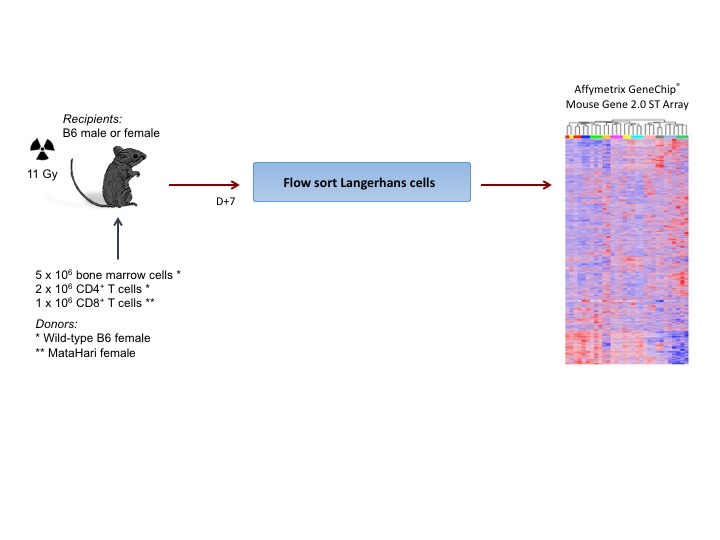
\includegraphics[width=22cm]{/cluster/project8/vyp/Winship_GVHD/vincent/GVHD/poster/figs/LangerhansCells.jpg}
    \end{center}
    %        \end{minipage}
    %  \begin{minipage}{20cm}
    \begin{itemize}
    \item Allogeneic BMT recipients (bone marrow B6 female donor and T cells from MataHari female donor B6 male recipient)
    \item Syngeneic BMT recipients (bone marrow and T cells from B6 female donor  B6 female recipient)
    \item Untreated recipient (B6 male)
    \end{itemize}
	%       \end{minipage}

	\begin{minipage}{0.6\textwidth}
	  \includegraphics[width=17cm]{/cluster/project8/vyp/Winship_GVHD/claire/results/syn_allo_bmt/figs/PCA_prettier.pdf}
	\end{minipage}
	\begin{minipage}{0.3\textwidth}
	  {\small             \begin{itemize}
    \item No particularly distinct clustering of samples evident
          \end{itemize}}
	\end{minipage}
  \end{block}
\vspace{3cm}

\begin{block}{ImmGen matching reveals hidden signals}

  {\bf BMT female vs naive male}

      \begin{minipage}{0.30\textwidth}
        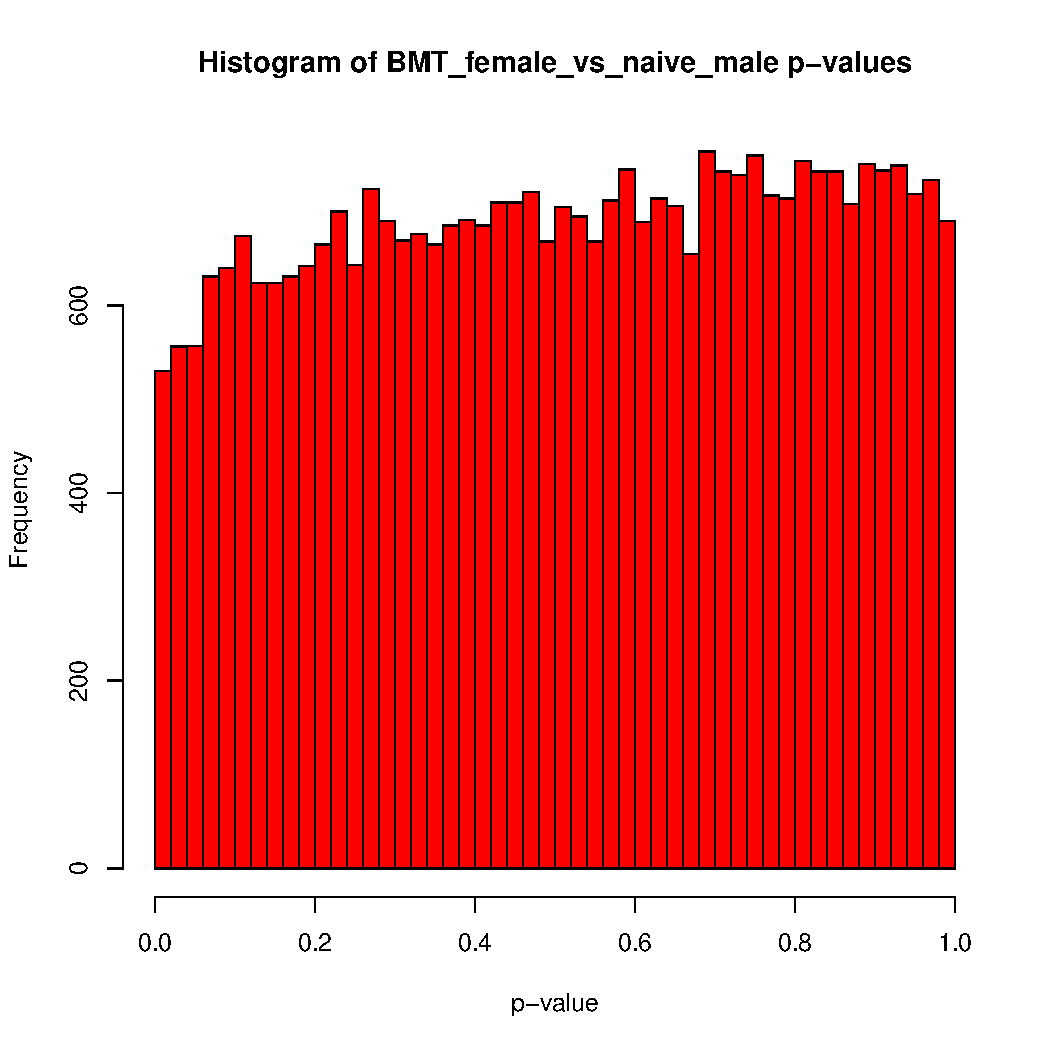
\includegraphics[width=10cm]{/cluster/project8/vyp/Winship_GVHD/claire/results/syn_allo_bmt/figs/BMT_female_vs_naive_male_histogram.pdf}
      \end{minipage}
  \hfill 
\begin{minipage}{0.30\textwidth}
        \includegraphics[width=10cm]{/cluster/project8/vyp/Winship_GVHD/claire/results/syn_allo_bmt/figs/BMT_female_vs_naive_male_coarse_module_association_graph.pdf}
      \end{minipage}
\hfill
\begin{minipage}{0.30\textwidth}
        \includegraphics[width=10cm]{/cluster/project8/vyp/Winship_GVHD/claire/results/syn_allo_bmt/figs/BMT_female_vs_naive_male_fine_module_association_graph.pdf}
      \end{minipage}
\begin{itemize}
\item Increased expression of coarse module 11 (cell cycle) genes in BMT female mouse 
\item Fine module 56 peak may suggest upregulation of one pathway/several closely related pathways 
\end{itemize}
\vspace{2cm}

{\bf BMT male vs naive male}
\vfill
\begin{minipage}{0.30\textwidth}
        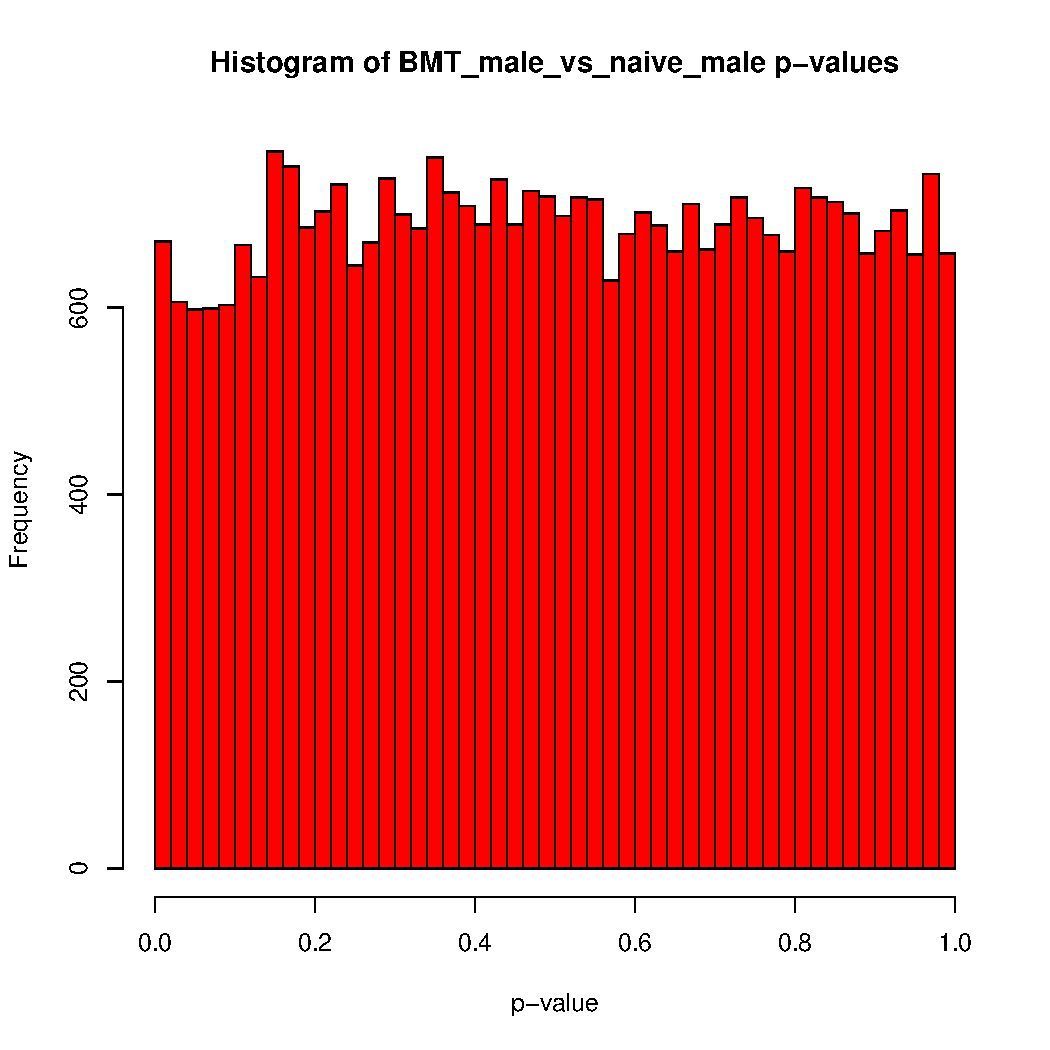
\includegraphics[width=10cm]{/cluster/project8/vyp/Winship_GVHD/claire/results/syn_allo_bmt/figs/BMT_male_vs_naive_male_histogram.pdf}
      \end{minipage}
  \hfill
      \begin{minipage}{0.30\textwidth}
        \includegraphics[width=10cm]{/cluster/project8/vyp/Winship_GVHD/claire/results/syn_allo_bmt/figs/BMT_male_vs_naive_male_coarse_module_association_graph.pdf}
      \end{minipage}
  \hfill
  \begin{minipage}{0.30\textwidth}
        \includegraphics[width=10cm]{/cluster/project8/vyp/Winship_GVHD/claire/results/syn_allo_bmt/figs/BMT_male_vs_naive_male_fine_module_association_graph.pdf}
  \end{minipage}
  \hfill
  \begin{itemize}
  \item Association with coarse module 34 - decrease in antigen processing/presentation in the BMT male
  \item Peak for coarse module 52 - contains interferon response genes  
    \end{itemize}
\end{block}
\vspace{3cm}

\begin{block}{Next steps}
\begin{itemize}
\item Need to identify T cell expression signature within lymph-node.
\item In vivo T cells rapidly migrate from lymph node - can be prevented using the drug Fingolimod (FTY720).
\item Confounding factor: are tissue specific interactions really key in GvHD or simply a reaction of T cells to a different signalling environment?
\item How can we better dissect the T-cell response to characterize the GvHD process?
\end{itemize}
\end{block}

\vspace{10cm}
\end{column}
\end{columns}
\end{frame}
\end{document}


%%%%%%%%%%%%%%%%%%%%%%%%%%%%%%%%%%%%%%%%%%%%%%%%%%%%%%%%%%%%%%%%%%%%%%%%%%%%%%%%%%%%%%%%%%%%%%%%%%%%
%%% Local Variables: 
%%% mode: latex
%%% TeX-PDF-mode: t
%%% End:
